\ejercicio
Probar que para todo $n \geq 3$ vale que:
\begin{enumerate}[label=\roman*)]
	\item La cantidad de diagonales de un polígono de $n$ lados es $\frac{n(n-3)}{2}$.\\
	      Ejercicio donde hay que encontrar una fórmula a partir de algún método \textit{creativo} para luego probar por inducción.\\
	      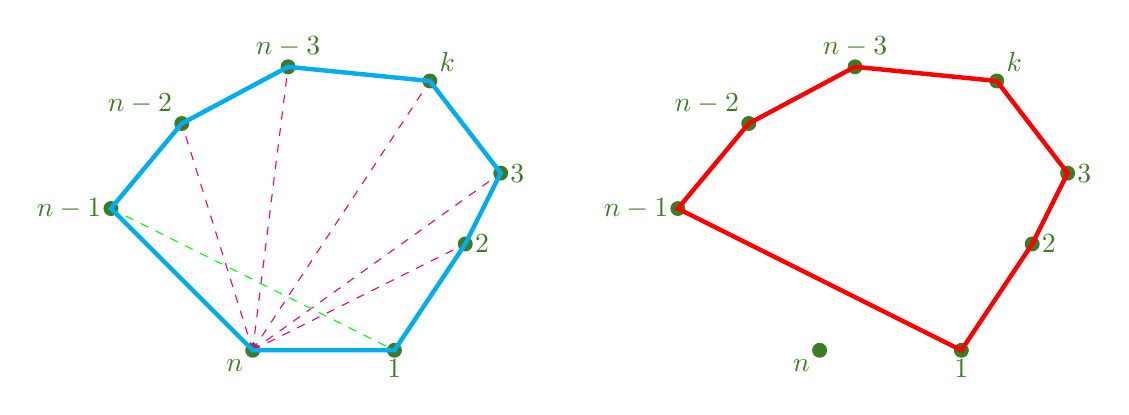
\begin{tikzpicture}[scale=0.9]
		      \coordinate (n) at (0,0);
		      \coordinate (1) at (2,0);
		      \coordinate (2) at (3,1.5);
		      \coordinate (3) at (3.5,2.5);
		      \coordinate (k) at (2.5,3.8);
		      \coordinate (n-3) at (0.5,4);
		      \coordinate (n-2) at (-1,3.2);
		      \coordinate (n-1) at (-2,2);

		      \foreach \point/\position in {n/below left, 1/below, 2/right, 3/right, k/above right, n-3/above, n-2/above left, n-1/left}
			      {
				      \fill[OliveGreen] (\point) circle (3pt) node [\position] {$\point$};
				      \draw[dashed, magenta] (n) -- (\point);
			      }
		      \draw[dashed, green] (n-1) -- (1);
		      \draw[ultra thick, cyan] (n) -- (1) -- (2) -- (3) -- (k) -- (n-3) -- (n-2) -- (n-1) -- cycle;

		      \begin{scope}[xshift=8cm]
			      \coordinate (n) at (0,0);
			      \coordinate (1) at (2,0);
			      \coordinate (2) at (3,1.5);
			      \coordinate (3) at (3.5,2.5);
			      \coordinate (k) at (2.5,3.8);
			      \coordinate (n-3) at (0.5,4);
			      \coordinate (n-2) at (-1,3.2);
			      \coordinate (n-1) at (-2,2);
			      \foreach \point/\position in {n/below left, 1/below, 2/right, 3/right, k/above right, n-3/above, n-2/above left, n-1/left}
				      {
					      \fill[OliveGreen] (\point) circle (3pt) node [\position] {$\point$};
				      }
		      \end{scope}

		      \draw[ultra thick, red] (n-1) -- (1) -- (2) -- (3) -- (k) -- (n-3) -- (n-2) -- (n-1) -- cycle;

	      \end{tikzpicture}\\
	      Se desprende del gráfico el siguiente razonamiento: En el polígono \cyan{cyan} de $n$ lados voy a tener una cantidad de
	      diagonales dada por la sucesión $d_n$. El polígono \red{rojo} me genera polígono que tiene un lado menos y
	      un lado menos, cantidad que viene determinada por $d_{n-1}$. Las líneas punteadas son las diagonales de $d_n$ que no estarán en
	      $d_{n-1}$. Ahora voy a encontrar una relación entre ambas sucesiones. Al sacan un lado pierdo las \magenta{diagonales} desde $2$ hasta $n-2$ que
	      serían $n - 3$ en total y además pierdo la {\color{green}diagonal} que conectan el vértice $1$ con el $n-1$:
	      $\cyan{d_n} = \red{d_{n-1}} + \green{1} +\magenta{n-2} = d_{n-1} + n - 1$
	      $\to {d_n = d_{n-1} + n - 1}$\\
	      Ahora inducción:\\
	      $p(n): d_n = \frac{n(n-3)}{2} \paratodo n \geq 3\\
		      \llave{l}{
		      \textit{Caso Base: } p(3) \V? \to \frac{3(3-3)}{2} = 0,\text{ lo cual es verdad para el triángulo.\Tilde}\\
		      \textit{Paso inductivo: } p(k) \text{ es verdadero para algún } k \en \enteros_{\geq 3} \entonces p(k+1) \V?\\
		      \textit{Hipótesis Inductiva: } d_k = \frac{k(k-3)}{2} \entonces d_{k+1} = \frac{(k+1)(k-2)}{ 2 } \\
		      d={k+1} \eqDef = d_k + k-1 \eqHI = \frac{k(k-3)}{2} + k-1 = \frac{k^2 - k - 2}{2} = \frac{(k-2)(k+1)}{2} \Tilde\\
		      }\\
	      $
	      Como $p(3) \y p(k) \y p(k+1)$ resultaron verdaderas, por el principio de inducción $p(n)$ es verdadera $\paratodo n \en \naturales_{\geq3}$

	\item la suma de los ángulos interiores de un polígono de $n$ lados es $\pi(n-2)$.\\
	      \begin{tikzpicture}[scale=0.9]
		      \coordinate (n) at (0,0);
		      \coordinate (1) at (2,0);
		      \coordinate (2) at (3.2,1.5);
		      \coordinate (3) at (3.7,2.8);
		      \coordinate (k) at (2.5,3.8);
		      \coordinate (n-3) at (0.5,4);
		      \coordinate (n-2) at (-1,3.2);
		      \coordinate (n-1) at (-2,2);

		      \foreach \point/\position in {n/below left, 1/below, 2/right, 3/right, k/above right, n-3/above, n-2/above left, n-1/left}
			      {
				      \fill[OliveGreen] (\point) circle (3pt) node [\position] {$\point$};
			      }
		      \draw[dashed, green] (n-1) -- (1);
		      \draw[ultra thick, cyan] (n) -- (1) -- (2) -- (3) -- (k) -- (n-3) -- (n-2) -- (n-1) -- cycle;


		      \draw[dashed, green] (n-1) -- (1);
		      \draw[ultra thick, cyan] (n) -- (1) -- (2) -- (3) -- (k) -- (n-3) -- (n-2) -- (n-1) -- cycle;

		      \pic [draw, angle eccentricity=1.5] {angle = 1--n--n-1};
		      \pic [draw, angle eccentricity=1.5] {angle = 2--1--n};
		      \pic [draw, angle eccentricity=1.5] {angle = 3--2--1};
		      \pic [draw, angle eccentricity=1.5] {angle = k--3--2};
		      \pic [draw, angle eccentricity=1.5] {angle = n-3--k--3};
		      \pic [draw, angle eccentricity=1.5] {angle = n-2--n-3--k};
		      \pic [draw, angle eccentricity=1.5] {angle = n-1--n-2--n-3};
		      \pic [draw, angle eccentricity=1.5] {angle = n--n-1--n-2};

		      \pic [draw, red, angle eccentricity=1.5, angle radius=1cm] {angle = n-1--1--n};
		      \pic [draw, red, angle eccentricity=1.5, angle radius=0.7cm] {angle = 1--n--n-1};
		      \pic [draw, red, angle eccentricity=1.5, angle radius=1cm] {angle = n--n-1--1};
	      \end{tikzpicture}\\
	      En este caso estoy generando la suma de los ángulos internos de 2 polígonos, uno con $\alpha_n$ de $n$ lados y otro con $n-1, \alpha_{n-1}$
	      Es más claro en este caso que al sacarle un lado, estoy robádo un triángulo que tiene como suma de sus ángulos internos $\pi$, entonces afirmo
	      $\alpha_{n+1} = \alpha_n + \pi $. Ahora pruebo por inducción lo pedido.
	      $p(n): \alpha_n = \pi(n-2) \paratodo n \geq 3$\\
	      $ \llave{l}{
			      \textit{Caso Base: } p(3) \V? \to \pi(3-2) = \pi, \text{ lo cual es verdad para el triángulo.\Tilde}\\
			      \textit{Paso inductivo: } p(k) \text{ es verdadero para algún } k \en \enteros_{\geq 3} \entonces p(k+1) \V?\\
			      \textit{Hipótesis Inductiva: } \alpha_k = \pi(k-2) \entonces \alpha_{k+1} = \pi(k-1) \\
			      \llaves{l}{
				      \alpha_k \eqDef = \alpha_{k+1} - \pi\\
				      \alpha_k \eqHI= \pi(k-2)\\
			      } \to \alpha_{k+1} = \pi(k-2) + \pi = \pi(k-1)\Tilde
		      }$\\
	      Como $p(3) \y p(k) \y p(k+1)$ resultaron verdaderas, por el principio de inducción $p(n)$ es verdadera $\paratodo n \en \naturales_{\geq3}$\\
\end{enumerate}
